%!TEX root = ../thesis.tex

\begin{savequote}[60mm]
	There's no reason to have a plan B\\
	because it distracts from plan A.
	\qauthor{Will Smith}
\end{savequote}

\chapter{Experimental results}\label{chapter:results}
	
	This chapter expands the previous one by verifying the usability of the Open LoRa Mesh.
	Particularly, it describes four experiments in which Open LoRa Mesh has been set up and tested, in order to record its rough performances.
	
	The following sections describe such experiments done with the available hardware in two particular locations: inside a building and in an open field.
	
	The first location is \textit{Archimedes Tower}\footnote{ For simplicity, pictures representing this location are taken from a publicly available online 3D model\newline (\url{https://3dwarehouse.sketchup.com/model/a4d327dd45162ee0557d96e459f19076/})} (\textit{Torre Archimede} in Italian), the building which houses the department of mathematics and computer science at the University of Padova, while the second place is the \textit{Mazzini Square}\footnote{ Images of this location in this thesis are taken from Google Maps and OpenStreetMap} (\textit{Piazza Mazzini} in Italian) in Monselice, a city in the south of Padova.
	
	These places have been chosen especially for their opposite characteristics.
	Archimedes Tower, in Figure~\ref{img:archimede_1}, is a 31m tall building which develops on seven levels above the ground and three underground levels\footnote{ \url{https://phaidra.cab.unipd.it/view/o:10783}}.
	On the other hand, Mazzini Square, in Figure~\ref{img:pzza_mazzini_1}, is an open space that allows an unobstructed view between nodes.
	
	An important remark that has to be done before describing these experiments is that they are not exhaustive.
	When thinking about the amount of possibilities in which nodes can be arranged, it is certain that more tests could have been executed.
	Such kind of system testing has to take in consideration also the surroundings of devices, since they communicate wirelessly.
	
	\begin{minipage}{0.5\textwidth}%
		\begin{figure}[H]
			\centering
			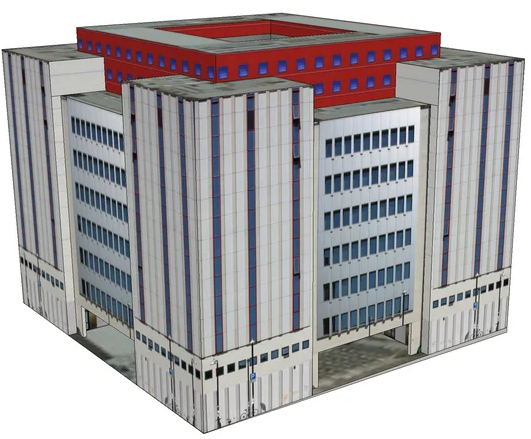
\includegraphics[width=\textwidth]{resources/img/chap5/archimede_1}
			\caption{3D model of Archimedes Tower}
			\label{img:archimede_1}
		\end{figure}
	\end{minipage}%
	\hfill%
	\begin{minipage}{0.5\textwidth}\raggedright
		\begin{figure}[H]
			\centering
			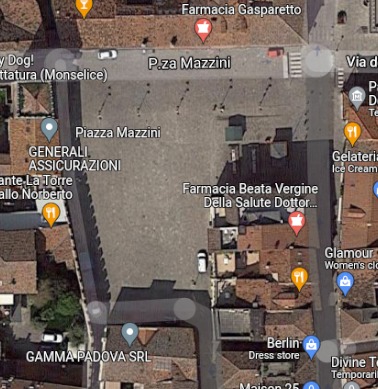
\includegraphics[width=.8\textwidth]{resources/img/chap5/pzza_mazzini_2}
			\caption{View from above of Mazzini Square}
			\label{img:pzza_mazzini_1}
		\end{figure}
	\end{minipage}%
	
	\section{Board placement}
	
		For these experiments, all four boards have been used to test the functionalities of the network.
		Placement of the boards is represented for both locations, respectively in Figure~\ref{img:archimede_2} for Archimedes Tower and in Figure~\ref{img:pzza_mazzini_2} for Mazzini Square.
		
		\begin{figure}[h]
			\centering
			\includegraphics[width=.6\textwidth]{resources/img/chap5/archimede_2}
			\caption{Placement of boards in Archimedes Tower}
			\label{img:archimede_2}
		\end{figure}
	
		Regarding Archimedes Tower, boards have been placed so that board \textbf{\textit{A}} is on the 6$^{th}$ floor, \textbf{\textit{B}} is on the 4$^{th}$ floor, \textbf{\textit{C}} is on the 2$^{nd}$ floor, \textbf{\textit{D}} is on the first underground level.
		All boards have been placed with the antenna facing the internal building courtyard.
		
		For Mazzini Square, on the other hand, boards have been placed so that they are directly visible to each other, almost one for each corner of the square.
		
		\begin{figure}[h]
			\centering
			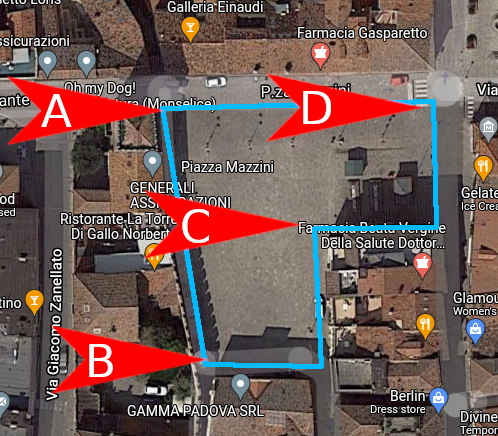
\includegraphics[width=.6\textwidth]{resources/img/chap5/pzza_mazzini_3}
			\caption{Placement of boards in Mazzini Square}
			\label{img:pzza_mazzini_2}
		\end{figure}
	
		These placements have been made so that boards do not have direct obstructions that can block the signal used in communicating.
		It can be considered as an ideal placement also because in this way nodes are all not that far from one another and their signal does not loose that much power.
		
		In both scenarios boards are tested as if they were part of a network of fixed devices, which, as explained in Section~\ref{sec:fixed_network}, is the best case scenario for Open LoRa Mesh.
	
	\section{Experiments}
	
		\subsection{Mesh creation}
		
		\subsection{Node addition}

		\subsection{Node removal}
		
		\subsection{Message propagation}
	
	\section{About the results}
	
		% When thinking about the first scenario where the network has been tested, it is possible to think of an optimal structure in which nodes are strategically placed to cover the entire area of the building:
	
	\section{Other possible experiments}
	
		Nothing is ever perfect, thus it is important to keep improving and test the work done.
		The aforementioned tests are not conclusive to declare Open LoRa Mesh ready for a ``\textit{production environment}'', where nodes can rely on the structure of the network to send their data.
		These tests only show that Open LoRa Mesh is a valid starting point to build upon and provide an interesting possibility in using LoRa as a transmission method.
		Also, as said earlier, the placement of nodes in the test can be considered ideal when thinking about signal strength and reach of LoRa antennas.
		
		A consideration on how other transmission methods would work compared to LoRa is talked about in Section~\ref{sec:other_transmission_methods}.